\documentclass[border=8pt]{standalone}
\usepackage[utf8]{inputenc}
\usepackage{tikz}
\usetikzlibrary{positioning}

\tikzset{
  entita/.style = {rectangle, draw, thick, fill=blue!8, minimum width=40mm, minimum height=34mm, font=\small},
  attr/.style   = {circle, draw, thick, fill=white, minimum size=5pt, inner sep=0},
  pk/.style     = {circle, draw, thick, fill=black, minimum size=5pt, inner sep=0},
  link/.style   = {thick},
  et/.style     = {font=\footnotesize}
}

\begin{document}
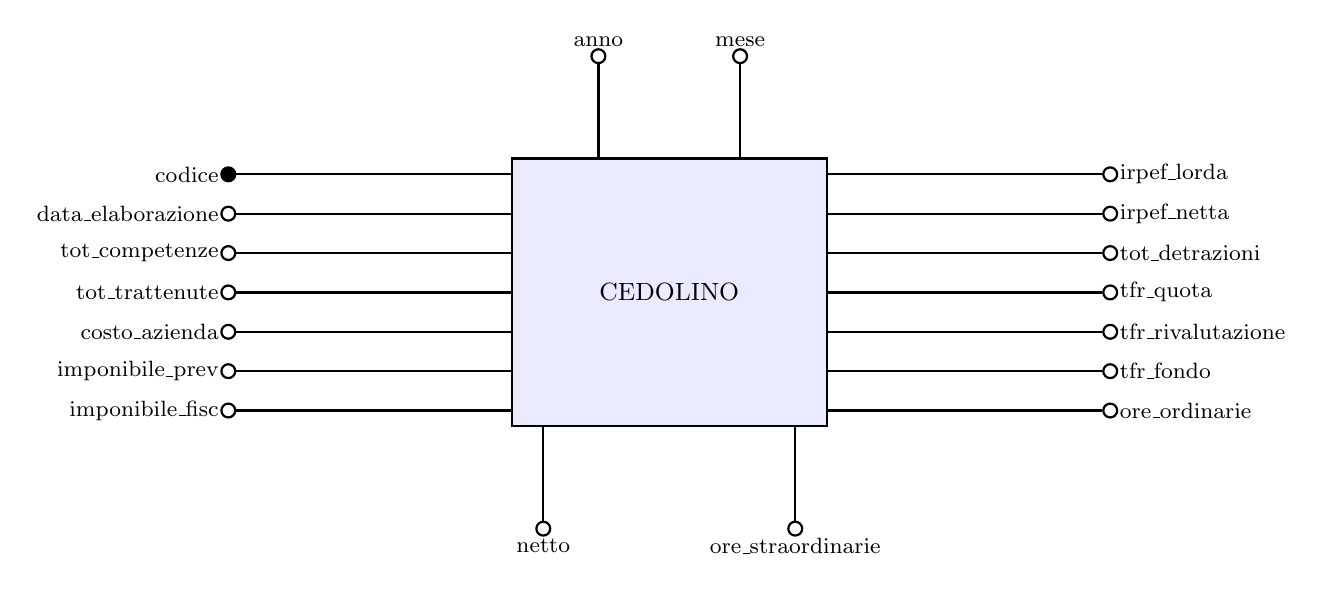
\begin{tikzpicture}

  \node[entita] (E) {CEDOLINO};

  % ---- lato sinistro (7) ----
  \node[pk]   (cod) at (-5.6, 1.5){}; \draw[link] (-2.0, 1.5)--(cod); \node[et,left] at (cod) {codice};
  \node[attr] (de)  at (-5.6, 1.0){}; \draw[link] (-2.0, 1.0)--(de);  \node[et,left] at (de)  {data\_elaborazione};
  \node[attr] (tc)  at (-5.6, 0.5){}; \draw[link] (-2.0, 0.5)--(tc);  \node[et,left] at (tc)  {tot\_competenze};
  \node[attr] (tt)  at (-5.6, 0.0){}; \draw[link] (-2.0, 0.0)--(tt);  \node[et,left] at (tt)  {tot\_trattenute};
  \node[attr] (ca)  at (-5.6,-0.5){}; \draw[link] (-2.0,-0.5)--(ca);  \node[et,left] at (ca)  {costo\_azienda};
  \node[attr] (ip)  at (-5.6,-1.0){}; \draw[link] (-2.0,-1.0)--(ip);  \node[et,left] at (ip)  {imponibile\_prev};
  \node[attr] (if)  at (-5.6,-1.5){}; \draw[link] (-2.0,-1.5)--(if);  \node[et,left] at (if)  {imponibile\_fisc};

  % ---- lato destro (7) ----
  \node[attr] (il) at (5.6, 1.5){}; \draw[link] (2.0, 1.5)--(il); \node[et,right] at (il) {irpef\_lorda};
  \node[attr] (in) at (5.6, 1.0){}; \draw[link] (2.0, 1.0)--(in); \node[et,right] at (in) {irpef\_netta};
  \node[attr] (td) at (5.6, 0.5){}; \draw[link] (2.0, 0.5)--(td); \node[et,right] at (td) {tot\_detrazioni};
  \node[attr] (tq) at (5.6, 0.0){}; \draw[link] (2.0, 0.0)--(tq); \node[et,right] at (tq) {tfr\_quota};
  \node[attr] (tr) at (5.6,-0.5){}; \draw[link] (2.0,-0.5)--(tr); \node[et,right] at (tr) {tfr\_rivalutazione};
  \node[attr] (tf) at (5.6,-1.0){}; \draw[link] (2.0,-1.0)--(tf); \node[et,right] at (tf) {tfr\_fondo};
  \node[attr] (oo) at (5.6,-1.5){}; \draw[link] (2.0,-1.5)--(oo); \node[et,right] at (oo) {ore\_ordinarie};

  % ---- lato superiore (2) ----
  \node[attr] (an) at (-0.9,3.0){}; \draw[link] (-0.9,1.7)--(an); \node[et,above] at (an) {anno};
  \node[attr] (me) at ( 0.9,3.0){}; \draw[link] ( 0.9,1.7)--(me); \node[et,above] at (me) {mese};

  % ---- lato inferiore (2) ----
  \node[attr] (nt) at (-1.6,-3.0){}; \draw[link] (-1.6,-1.7)--(nt); \node[et,below] at (nt) {netto};
  \node[attr] (os) at ( 1.6,-3.0){}; \draw[link] ( 1.6,-1.7)--(os); \node[et,below] at (os) {ore\_straordinarie};

\end{tikzpicture}
\end{document}
